\documentclass{article}
\usepackage[margin=1in]{geometry} % For setting page margins
\usepackage{amsmath}
\usepackage{amssymb} % For math symbols and equations
\usepackage{graphicx} % For including images
\usepackage{hyperref} 
\usepackage{enumitem}
\usepackage{float}
\usepackage{listings}
\usepackage{xcolor}
\usepackage{caption}

\renewcommand{\thesection}{(\alph{section})}
\renewcommand{\thesubsection}{\arabic{subsection}.}

\lstdefinestyle{matlabstyle}{
    language=Matlab,              % Specify the language
    basicstyle=\ttfamily\footnotesize\color{black}, % Code font
    keywordstyle=\color{blue}\bfseries, % Keywords in blue
    stringstyle=\color{orange},    % Strings in green
    commentstyle=\color{magenta}, % Comments in magenta
    numbers=left,                 % Line numbers on the left
    numberstyle=\tiny\color{black},% Line number style
    stepnumber=1,                 % Line number increment
    breaklines=true,              % Line breaking
    frame=single,                 % Border around code
    backgroundcolor=\color{white},
    tabsize=4,                    % Tab size
    showstringspaces=false,       % Don't show spaces in strings
}

\begin{document}

\title{
    \begin{tabular}{@{}l@{}}
        \textbf{Class:} Robust Multivariate Control \\ 
        \textbf{Professor:} Dr. Sean Humbert \\ 
        \textbf{TAs:} Santosh Chaganti \\ 
        \textbf{Student:} Steve Gillet \\ 
        \textbf{Date:} \today \\ 
        \textbf{Assignment:} Final Project \\
    \end{tabular}
}

\author{}
\date{}

\maketitle

\section*{Project Overview}

The original project was for the robust inner loop control of a 6-DOF Micro-Helicopter described in the problem statement below. \\

\textit{For this project you will synthesize a series of inner loop controllers using $H_{\infty}$ and $\mu$-synthesis techniques for an 11-state rotary wing micro-helicopter and analyze their robustness properties. The state vector is given by $x = [u, v, p, q, \phi, \theta, a_s, b_s, w, r, r_{fb}]^T$. The variables $u$, $v$, $w$ are the vehicle translational velocities along the vehicle's longitudinal, lateral, and vertical body axis, $p$, $q$, $r$ are the vehicle roll, pitch, and yaw rate respectively, $\phi$ and $\theta$ are the roll and pitch attitude, $a_s$ and $b_s$ are the rotor dynamics states (flap of the rotor relative to the body), and $r_{fb}$ is the washed out yaw rate, a filtering state associated with on-board yaw rate feedback. The control input vector is $u = [\delta_{\text{long}}, \delta_{\text{lat}}, \delta_{\text{ped}}]^T$, corresponding to the longitudinal cyclic, the lateral cyclic, and the tail rotor inputs. The outputs available for feedback are the pitch and roll attitude $\theta$ and $\phi$, and the washed out yaw rate $r_{fb}$. The equations of motion linearized about hover are given in the MATLAB m-file on the Canvas website.}

\textit{The objective of the project is to design a controller to ensure robust command tracking of $\theta_r \rightarrow \theta$ and $\phi_r \rightarrow \phi$ for the reference $r=\begin{bmatrix} \theta_r & \phi_r \end{bmatrix}^T$ in the presence of a structured multiplicative input uncertainty.} \\

I chose to do a 2-wheeled self-balancing robot with different drive instead because I had attempted one as an undergrad and I've been thinking about it a while.

The dynamics are actually a bit more simple for the self-balancing robot, essentially a cart inverted pendulum with the differential drive, but I believe that I can accomplish the same objectives by changing a few of the specifics such as the input to output channels of interest.
I'll go into detail of the changes as they come up.
Below is an overview of the system and a derivation of the state-space model.

\section*{Dynamics of a 2-Wheeled Self-Balancing Robot with Differential Drive}

This section derives the equations of motion for a 2-wheeled self-balancing robot capable of moving and turning in a 2D plane. The robot is modeled as an inverted pendulum mounted on a wheeled base, with separate torque inputs applied to each wheel to enable differential drive. The nonlinear dynamics are derived using Newtonian mechanics, linearized around the upright equilibrium, and expressed in state-space form.

\subsection{System Description and Variables}

The robot consists of a body with mass \( M \), whose center of mass is located at a distance \( l \) above the wheel axle, and two wheels with total mass \( m \), each of radius \( R \). The wheels are separated by a distance \( d \). Separate torques \( \tau_l \) and \( \tau_r \) are applied to the left and right wheels, respectively, enabling both translation and rotation.

The state variables are:
\begin{itemize}
    \item \( \theta \): Tilt angle of the body from the vertical (upright at \( \theta = 0 \)).
    \item \( \dot{\theta} \): Angular velocity of the tilt.
    \item \( \psi \): Yaw angle, defining the robot's orientation in the 2D plane.
    \item \( \dot{\psi} \): Yaw rate (angular velocity about the vertical axis).
    \item \( v \): Forward velocity of the robot along its heading (direction of \( \psi \)).
\end{itemize}

The state vector is:
\begin{equation}
    z = \begin{bmatrix} \theta & \dot{\theta} & \psi & \dot{\psi} & v \end{bmatrix}^T
\end{equation}

The control inputs are the torques:
\begin{equation}
    u = \begin{bmatrix} \tau_l & \tau_r \end{bmatrix}^T
\end{equation}

Alternatively, inputs can be expressed as average and differential torques:
\begin{equation}
    \tau_{\text{avg}} = \frac{\tau_l + \tau_r}{2}, \quad \tau_{\text{diff}} = \frac{\tau_r - \tau_l}{2}
\end{equation}

Constants include gravitational acceleration \( g = 9.81 \, \text{m/s}^2 \) and the moment of inertia \( I_\psi \) of the robot about the vertical axis.

\subsection{Nonlinear Equations of Motion}

The dynamics are derived by considering the translational motion of the system, the rotational motion of the pendulum-like body, and the yaw motion due to differential torques.

\subsubsection{Translational Motion}

The robot moves in the direction of its heading (aligned with \( \psi \)). The force from each wheel is \( F_l = \frac{\tau_l}{R} \) and \( F_r = \frac{\tau_r}{R} \). The total force along the heading is:
\begin{equation}
    F = F_l + F_r = \frac{\tau_l + \tau_r}{R}
\end{equation}

Summing forces in the direction of motion, accounting for the pendulum's effect:
\begin{equation}
    (M + m) \dot{v} + m l \ddot{\theta} \cos \theta - m l \dot{\theta}^2 \sin \theta = \frac{\tau_l + \tau_r}{R}
\end{equation}
Here:
\begin{itemize}
    \item \( (M + m) \dot{v} \): Total mass times acceleration along the heading.
    \item \( m l \ddot{\theta} \cos \theta \): Horizontal component of the pendulum's acceleration.
    \item \( - m l \dot{\theta}^2 \sin \theta \): Centripetal force term.
\end{itemize}

\subsubsection{Rotational Motion (Pendulum)}

For the body, summing torques about its center of mass (or using force balance in the horizontal direction):
\begin{equation}
    m l \ddot{\theta} + m g \sin \theta + m \dot{v} \cos \theta = 0
\end{equation}
Here:
\begin{itemize}
    \item \( m l \ddot{\theta} \): Rotational acceleration.
    \item \( m g \sin \theta \): Gravity torque.
    \item \( m \dot{v} \cos \theta \): Coupling with the base's acceleration.
\end{itemize}

\subsubsection{Yaw Motion}

The differential torque causes rotation about the vertical axis. The torque about the center of the robot is:
\begin{equation}
    \tau_\psi = \frac{d}{2} (F_r - F_l) = \frac{d}{2} \left( \frac{\tau_r}{R} - \frac{\tau_l}{R} \right) = \frac{d}{2 R} (\tau_r - \tau_l)
\end{equation}
The yaw dynamics are:
\begin{equation}
    I_\psi \ddot{\psi} = \frac{d}{2 R} (\tau_r - \tau_l)
\end{equation}
where \( I_\psi \) is the moment of inertia about the vertical axis.

\subsection{Linearization Around the Equilibrium Point}

Linearize around the equilibrium: \( \theta = 0 \), \( \dot{\theta} = 0 \), small \( \dot{\psi} \), and constant \( v \). Approximations:
\begin{itemize}
    \item \( \sin \theta \approx \theta \)
    \item \( \cos \theta \approx 1 \)
    \item \( \dot{\theta}^2 \approx 0 \)
\end{itemize}

The equations become:

1. **Translational**:
\begin{equation}
    (M + m) \dot{v} + m l \ddot{\theta} = \frac{\tau_l + \tau_r}{R}
\end{equation}

2. **Rotational**:
\begin{equation}
    m l \ddot{\theta} + m g \theta + m \dot{v} = 0
\end{equation}

3. **Yaw**:
\begin{equation}
    I_\psi \ddot{\psi} = \frac{d}{2 R} (\tau_r - \tau_l)
\end{equation}

\subsection{Solving for Accelerations}

Solve for \( \ddot{\theta} \), \( \dot{v} \), and \( \ddot{\psi} \):

From (11):
\begin{equation}
    \dot{v} = -l \ddot{\theta} - g \theta
\end{equation}

Substitute into (10):
\begin{equation}
    (M + m) (-l \ddot{\theta} - g \theta) + m l \ddot{\theta} = \frac{\tau_l + \tau_r}{R}
\end{equation}
\begin{equation}
    -(M + m) l \ddot{\theta} - (M + m) g \theta + m l \ddot{\theta} = \frac{\tau_l + \tau_r}{R}
\end{equation}
\begin{equation}
    -M l \ddot{\theta} - (M + m) g \theta = \frac{\tau_l + \tau_r}{R}
\end{equation}
\begin{equation}
    M l \ddot{\theta} + (M + m) g \theta = -\frac{\tau_l + \tau_r}{R}
\end{equation}
\begin{equation}
    \ddot{\theta} = -\frac{(M + m) g}{M l} \theta - \frac{1}{M l R} (\tau_l + \tau_r)
\end{equation}

Substitute back into (13):
\begin{equation}
    \dot{v} = -l \left( -\frac{(M + m) g}{M l} \theta - \frac{1}{M l R} (\tau_l + \tau_r) \right) - g \theta
\end{equation}
\begin{equation}
    \dot{v} = \frac{(M + m) g}{M} \theta + \frac{1}{M R} (\tau_l + \tau_r) - g \theta
\end{equation}
\begin{equation}
    \dot{v} = \frac{m g}{M} \theta + \frac{1}{M R} (\tau_l + \tau_r)
\end{equation}

From (12):
\begin{equation}
    \ddot{\psi} = \frac{d}{2 I_\psi R} (\tau_r - \tau_l)
\end{equation}

Using \( \tau_{\text{avg}} = \frac{\tau_l + \tau_r}{2} \), \( \tau_{\text{diff}} = \frac{\tau_r - \tau_l}{2} \):
\begin{equation}
    \tau_l + \tau_r = 2 \tau_{\text{avg}}, \quad \tau_r - \tau_l = 2 \tau_{\text{diff}}
\end{equation}
Rewrite (18) and (20):
\begin{equation}
    \ddot{\theta} = -\frac{(M + m) g}{M l} \theta - \frac{2}{M l R} \tau_{\text{avg}}
\end{equation}
\begin{equation}
    \dot{v} = \frac{m g}{M} \theta + \frac{2}{M R} \tau_{\text{avg}}
\end{equation}
\begin{equation}
    \ddot{\psi} = \frac{d}{I_\psi R} \tau_{\text{diff}}
\end{equation}

\subsection{State-Space Model}

The state-space representation is:
\begin{equation}
    \dot{z} = A z + B u
\end{equation}
where \( z = [\theta, \dot{\theta}, \psi, \dot{\psi}, v]^T \), \( u = [\tau_{\text{avg}}, \tau_{\text{diff}}]^T \), and:
\begin{equation}
    A = \begin{bmatrix}
        0 & 1 & 0 & 0 & 0 \\
        -\frac{(M + m) g}{M l} & 0 & 0 & 0 & 0 \\
        0 & 0 & 0 & 1 & 0 \\
        0 & 0 & 0 & 0 & 0 \\
        \frac{m g}{M} & 0 & 0 & 0 & 0
    \end{bmatrix}, \quad
    B = \begin{bmatrix}
        0 & 0 \\
        -\frac{2}{M l R} & 0 \\
        0 & 0 \\
        0 & \frac{d}{I_\psi R} \\
        \frac{2}{M R} & 0
    \end{bmatrix}
\end{equation}

This model captures the unstable balancing dynamics (\( \theta \)) and the decoupled yaw dynamics (\( \psi \)), driven by the average and differential torques.

\section{}
\textit{Construct the corresponding block diagram and formulate the generalized plant with the relevant uncertainty and performance weighting functions to achieve the desired command tracking behavior. Note that the output as prescribed has three states; you will include the $r_{fb}$ state in the reference input as well so that the $G$ and $K$ matrix transfer functions are square. However from the design perspective we are only interested in the performance in the $\theta_r \rightarrow \theta$ and $\phi_r \rightarrow \phi$ channels.}

I will do the same thing for my model except that there are just the two measurable, feedback-available, states of interest $\theta$ and $\psi$, so we will look at the performance in the $\theta_r \rightarrow \theta$ and $\psi_r \rightarrow \psi$ channels.

Here is the block diagram for a multiplicative input uncertainty model:

\begin{figure}[H]
    \centering
    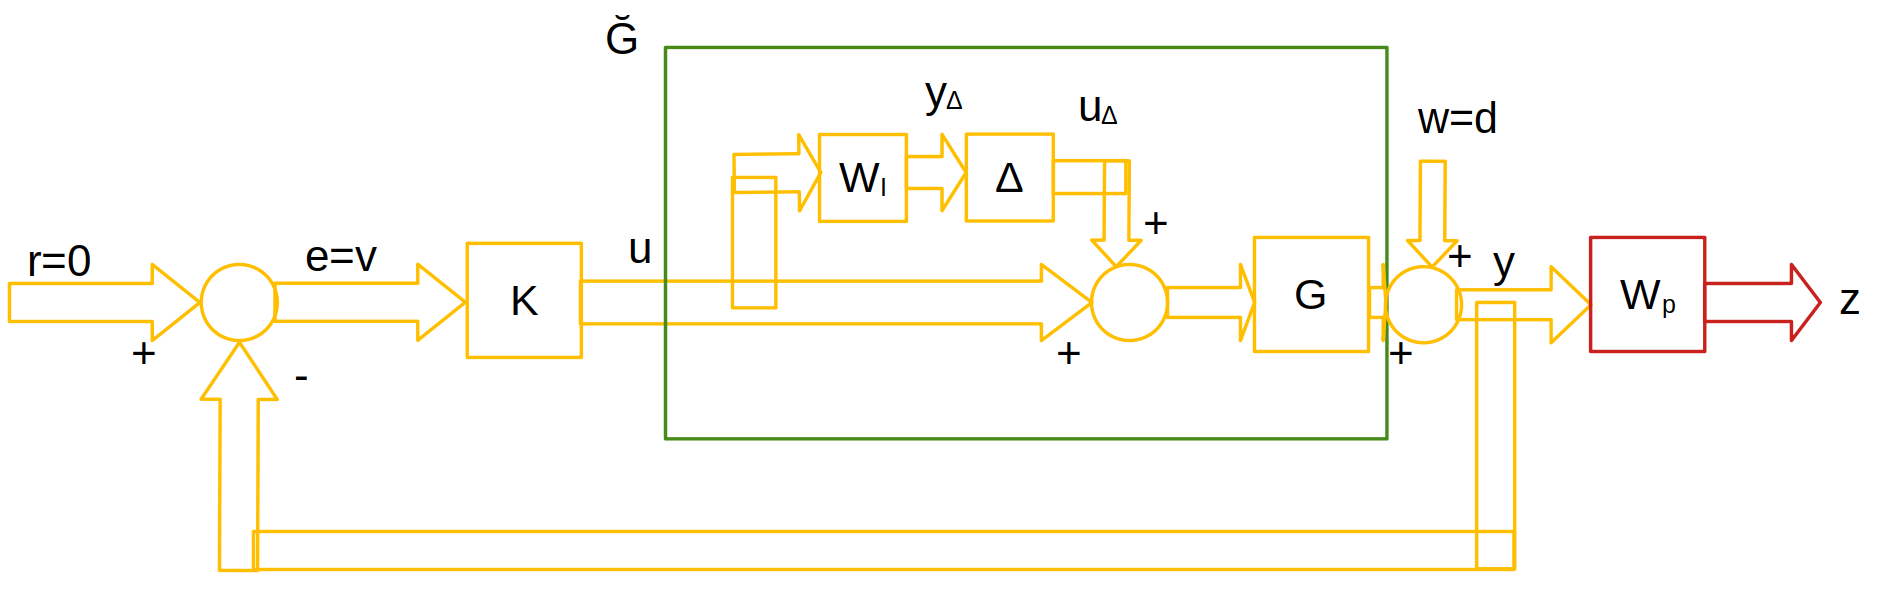
\includegraphics[width=0.8\textwidth]{blockDiagram.png}
    \caption{Block diagram of the system with multiplicative input uncertainty.}
    \label{fig:blockDiagram}    
\end{figure}

Here is the generalized plant formulation:

Putting $y_\Delta$, $z$, and $v$ in terms of $u_\Delta$, $w$, and $u$:

\begin{align}
    y_\Delta &= W_I u \\
    z &= W_P [w + G(u_\Delta + u)] \\
    v &= -[w + G(u_\Delta + u)] 
\end{align}

$\begin{bmatrix} y_\Delta \\ z \\ v \end{bmatrix} = \begin{bmatrix} 0 & 0 & W_I \\ W_P G & W_P & W_P G \\ -G & -I & -G \end{bmatrix} \begin{bmatrix} u_\Delta \\ w \\ u \end{bmatrix}$

\section{}
\textit{Synthesize a $H_{\infty}$ controller and analyze its nominal performance via singular value plots of the open loop transfer functions $G$, $G K$ and closed loop transfer functions $S_o$, $T_b$ and performance weight $W_p$. Provide plots of step responses in $\theta_r \to \theta$ and $\phi_r \to \phi$ and the output disturbance quantities $d_\theta \to \theta$ and $d_\phi \to \phi$ for a disturbance vector $d_o = \begin{bmatrix} d_\theta & d_\phi \end{bmatrix}^T$. Comment on the performance of your design in terms of its bandwidth, tracking error, and disturbance rejection capabilities.}

I designeed the $H_\infty$ controller using 'sysic' and 'hinfsyn' in Matlab as shown in the code below.

\begin{lstlisting}[style=matlabstyle]
systemnames = 'G Wp';
inputvar = '[w(2); u(2)]';
outputvar = '[Wp; -G-w]';
input_to_G = '[u]';
input_to_Wp = '[w + G]';
sysoutname = 'P';
sysic;
P = minreal(ss(P));


[K, CL, gamma, info] = hinfsyn(P,nOut,nIn,'method','ric','Tolgam',1e-3,'DISPLAY','on');        
\end{lstlisting}

I used a generic weighting function that we had used in class before, it basically weighs each channel the same and decays as the frequency increases.

\begin{lstlisting}[style=matlabstyle]
s = tf('s');
Wp_theta = (s/100 + 1)/(s + 1*0.01);  % Low-frequency gain ~100, bandwidth ~1 rad/s
Wp_psi = (s/100 + 1)/(s + 1*0.01);    % Adjust parameters later
Wp = blkdiag(Wp_theta, Wp_psi);
Wp = ss(Wp);    
\end{lstlisting}

Then I plotted $G$, $GK$, $S_O$, $T_O$, and $W_P$ using the 'sigma' function.

\begin{figure}
    \centering
    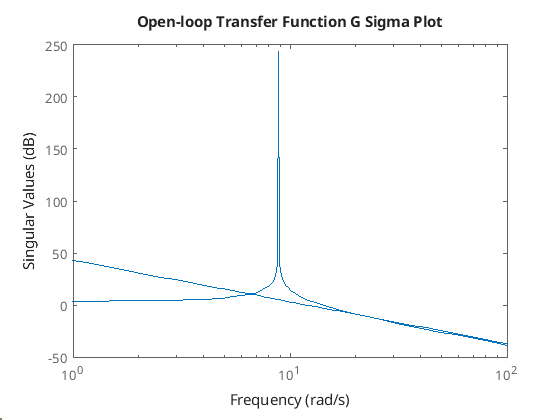
\includegraphics[width=0.8\textwidth]{sigmaG.png}
    \caption{Singular values of G.}
    \label{fig:sigmaG}
\end{figure}

\begin{figure}
    \centering
    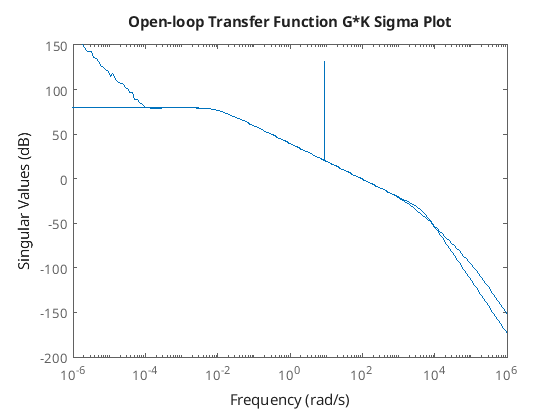
\includegraphics[width=0.8\textwidth]{sigmaGK.png}
    \caption{Singular values of GK.}
    \label{fig:sigmaGK}
\end{figure}

\begin{figure}
    \centering
    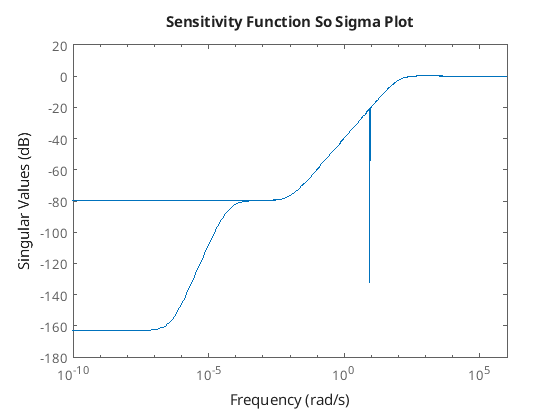
\includegraphics[width=0.8\textwidth]{sigmaSo.png}
    \caption{Singular values of So.}
    \label{fig:sigmaSo}
\end{figure}

\begin{figure}
    \centering
    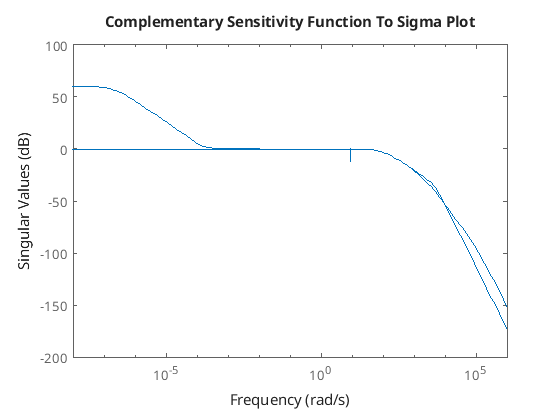
\includegraphics[width=0.8\textwidth]{sigmaTo.png}
    \caption{Singular values of To.}
    \label{fig:sigmaTo}
\end{figure}

\begin{figure}
    \centering
    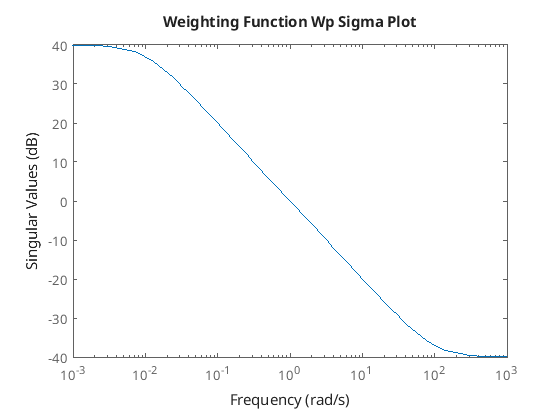
\includegraphics[width=0.8\textwidth]{sigmaWp.png}
    \caption{Singular values of Wp.}
    \label{fig:sigmaWp}
\end{figure}

Then I plotted the responses of the closed loop system to step inputs in the reference and disturbance channels.

\begin{figure}
    \centering
    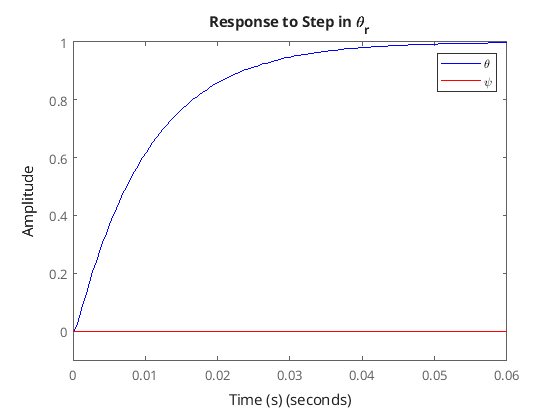
\includegraphics[width=0.8\textwidth]{stepTheta.png}
    \caption{Step response for theta.}
    \label{fig:stepTheta}
\end{figure}

\begin{figure}
    \centering
    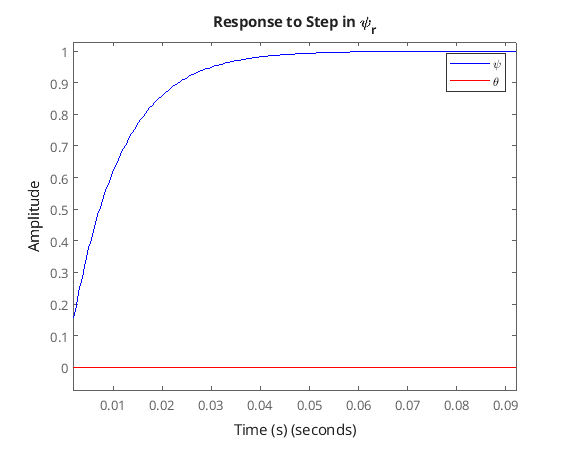
\includegraphics[width=0.8\textwidth]{stepPsi.png}
    \caption{Step response for psi.}
    \label{fig:stepPsi}
\end{figure}

\begin{figure}
    \centering
    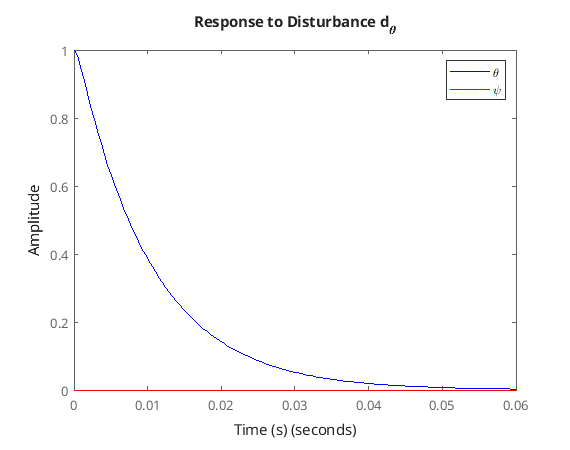
\includegraphics[width=0.8\textwidth]{stepDtheta.png}
    \caption{Step response for theta disturbance.}
    \label{fig:stepDtheta}
\end{figure}

\begin{figure}
    \centering
    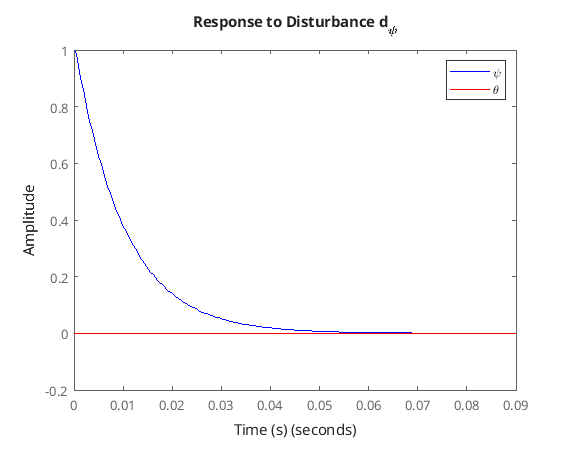
\includegraphics[width=0.8\textwidth]{stepDpsi.png}
    \caption{Step response for psi disturbance.}
    \label{fig:stepDpsi}
\end{figure}

The closed loop bandwidth is about 90 rad/s, the tracking error is 6\% up to 6.28 rad/s, and the settling time is 0.03 seconds for disturbance rejection. 

\section{}
\textit{Update the generalized plant to include a diagonal structured complex uncertainty with a relative weight of $w_i(s) = \frac{s + 0.2}{0.5 s + 1}$ in each channel. Assume $\|\Delta\|_{\infty} \leq 1$, and compute the upper and lower bounds on the structured singular value for the controller obtained above, and determine the margins $\left(1 / \mu_{\text{peak}}\right)$ on robust stability and robust performance. Provide an iteration on the performance weighting function to obtain improved margins. Note that if you are using only $\theta$, $\phi$, and $r_{fb}$ as outputs, I don't expect you to achieve robust performance for the given uncertainty profiles, but rather use these tools to assess how much uncertainty your design can tolerate. Again provide plots of step responses in $\theta$ and $\phi$ and the disturbance channels and comment on the performance of your design.}


\end{document}